\subsection{Why is Aging a Problem?}

\begin{frame}[c]{Corona Deaths correlate with Age}
    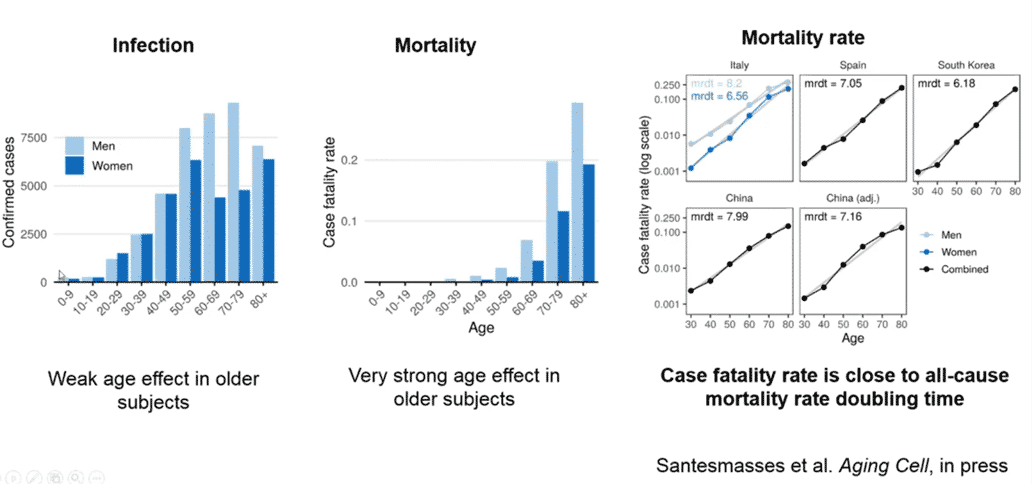
\includegraphics[width=\textwidth]{corona_death_rates} \\
    Source: \cite{10.1111/acel.13230} \\
    \pnote{
        Corona deaths correlate strongly with age \\
        \par
        Infection is mostly detected through symptoms \\
        no detection of many infections in aged <20
        \par
        Next: Treating Corona with Senolytics
    }
\end{frame}


\begin{frame}[c]{Treating Corona with Senolytics (anti-aging approach) in Mice}
    % trim = l b r t
    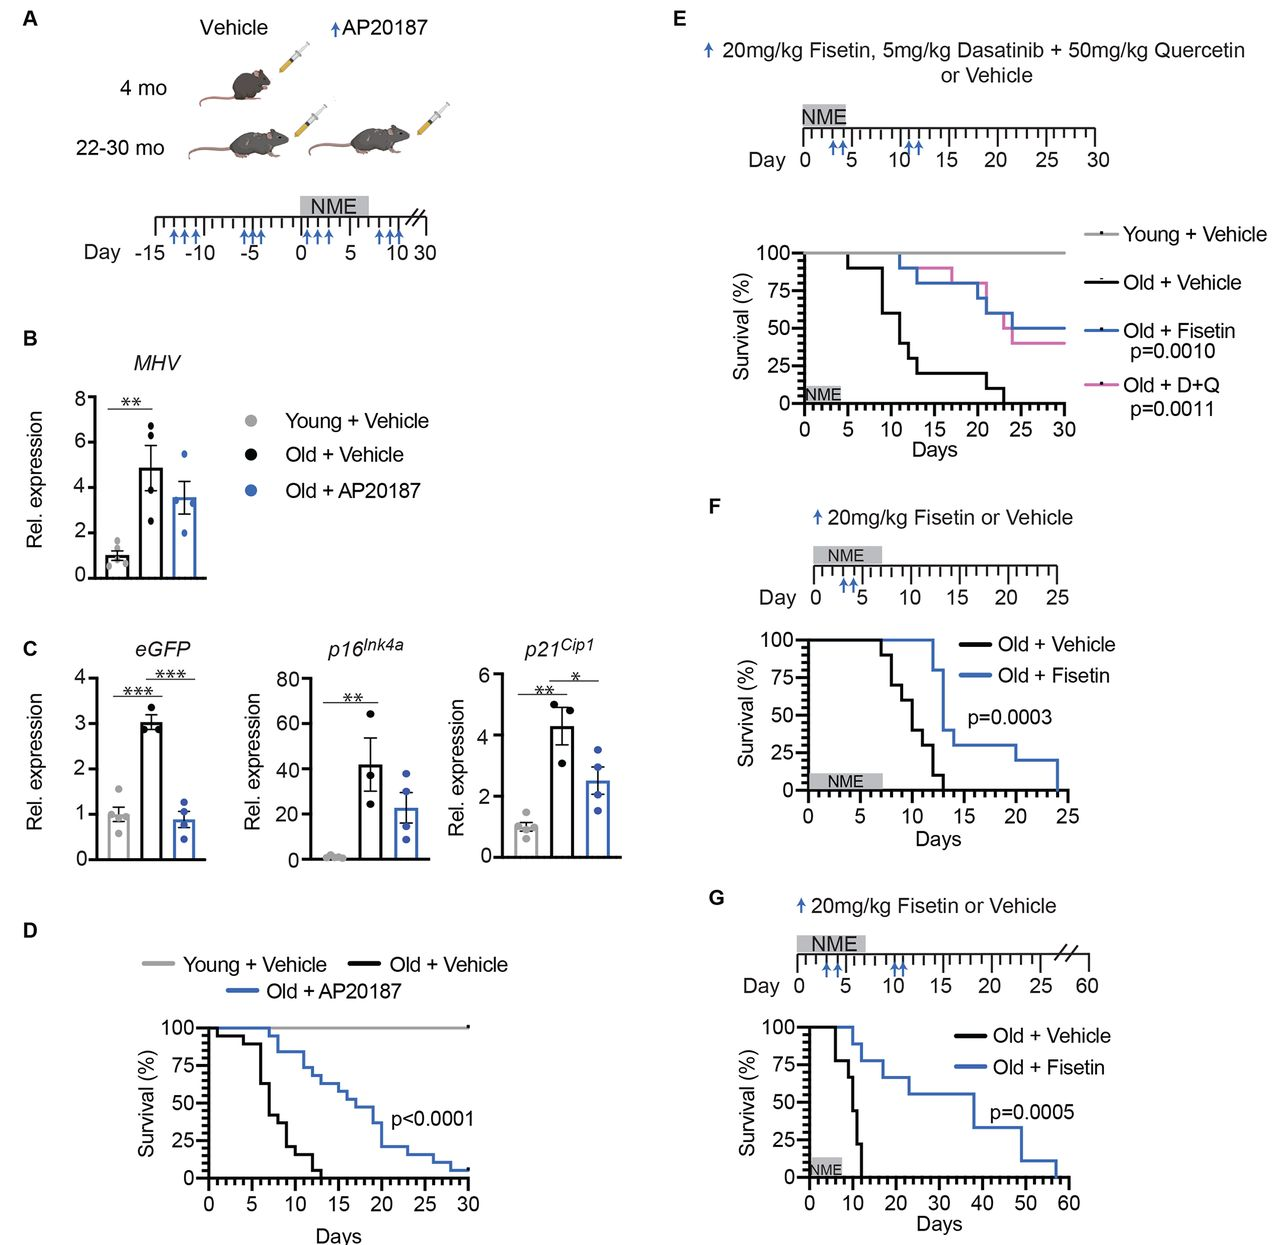
\includegraphics[width=\textwidth,clip,trim=170 180 0 50]{mice_corona} \\
    Source: \cite{camell2021senolytics} \\
    \pause
    Hypothesis: They die due to old age, not Corona!
    \pnote{
        Mortality-Comparison after corona infection \\
        NME = Guaranteed Infection \\
        These were very old Mice \\
        Treatment with senolytics helps them \\
        overcome corona, making seem younger \\
        \par
        Fisetin as well as Dasatinib and Quercetin \\
        are well-established senolytics \\
        NME = Normal Microbial Experience;   \\
              pathogen infection/exposure
    }
\end{frame}


\begin{frame}[c]{All causes for Death correlate with Age}
    \large
    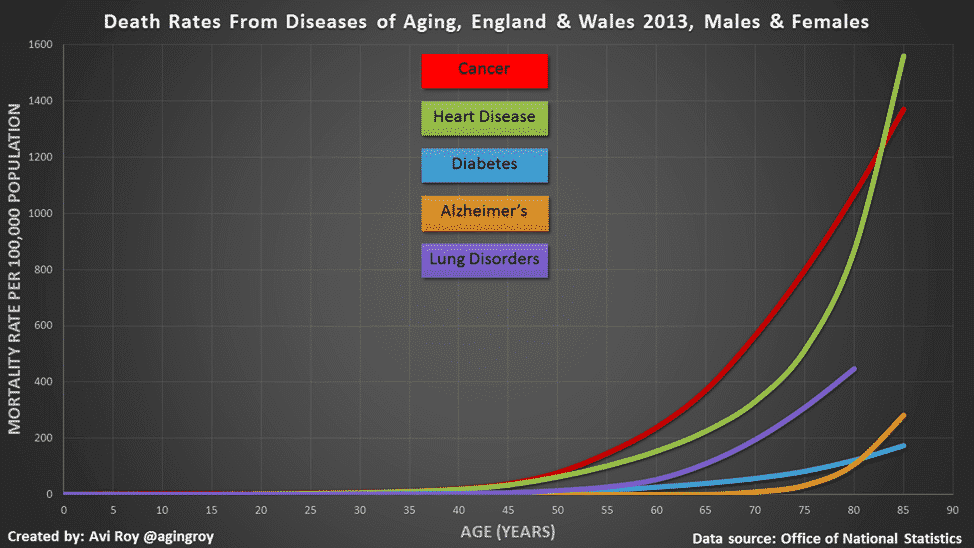
\includegraphics[width=\textwidth]{death_rates} \\
    Same with all other primary causes!
    \pnote{
        Similarly, these diseases are not \\
        life-threathening when young! only old \\
    }
\end{frame}


\begin{frame}[c]{Slowing aging has incredible potential}
    \large
    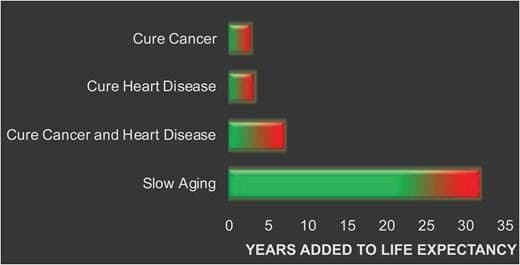
\includegraphics[width=\textwidth]{potential} \\
    Source: \cite{10.1093/ppar/prz022} \\
    \pause
    And yet it receives less than 1/100th of Funding!
    \pnote{
        Curing Cancer completely: about 4Y \\
        Curing Heart Diseases: about 4.5Y \\
        Curing both: about 7Y \\
        \par
        Slowing down aging: by the amount slowed down \\
        also healthspan, not just lifespan! \\
    }
\end{frame}


